\documentclass[aspectratio=169]{beamer}
\usetheme{Madrid}
\usecolortheme{default}

\usepackage{amsmath}
\usepackage{amsfonts}
\usepackage{amssymb}
\usepackage{graphicx}
\usepackage{tikz}
\usepackage{pgfplots}
\pgfplotsset{compat=1.18}

% Title page info
\title{Importance Sampling in BRDF Evaluation}
\subtitle{Advanced Monte Carlo Techniques for Realistic Rendering}
\author{Your Name}
\institute{BUET CSE 409: Computer Graphics}
\date{\today}

\begin{document}

% Frame 1: Title Slide
\begin{frame}
    \titlepage
    \begin{center}
        \vspace{0.5cm}
        \textcolor{blue}{\large Exploratory Presentation on Advanced Graphics Topics}
    \end{center}
\end{frame}

% Frame 2: Problem Statement
\begin{frame}{The Rendering Challenge}
    \begin{columns}
        \begin{column}{0.6\textwidth}
            \textbf{The Problem:}
            \begin{itemize}
                \item<1-> How much light reaches the camera from a surface?
                \item<2-> Need to integrate over \textbf{all possible light directions}
                \item<3-> BRDF describes surface reflection properties
                \item<4-> Analytical solution often impossible
            \end{itemize}
            
            \vspace{0.5cm}
            \textbf{The Integral:}
            \begin{align}
                L_o &= \int_{\Omega} f_r(\omega_i, \omega_o) L_i(\omega_i) \cos\theta_i d\omega_i
            \end{align}
        \end{column}
        \begin{column}{0.4\textwidth}
            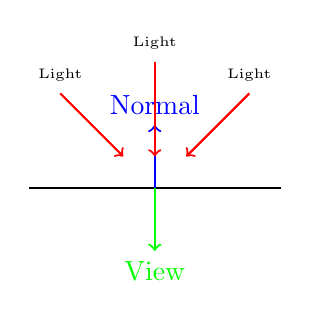
\begin{tikzpicture}[scale=0.8]
                % Surface
                \draw[thick] (-2,0) -- (2,0);
                \draw[->, thick, blue] (0,0) -- (0,1) node[above] {Normal};
                
                % Light rays
                \draw[->, red, thick] (-1.5,1.5) -- (-0.5,0.5);
                \draw[->, red, thick] (0,2) -- (0,0.5);
                \draw[->, red, thick] (1.5,1.5) -- (0.5,0.5);
                
                % View direction
                \draw[->, green, thick] (0,0) -- (0,-1) node[below] {View};
                
                % Labels
                \node at (-1.5,1.8) {\tiny Light};
                \node at (0,2.3) {\tiny Light};
                \node at (1.5,1.8) {\tiny Light};
            \end{tikzpicture}
        \end{column}
    \end{columns}
\end{frame}

% Frame 3: BRDF Basics
\begin{frame}{Bidirectional Reflectance Distribution Function (BRDF)}
    \begin{columns}
        \begin{column}{0.5\textwidth}
            \textbf{What is BRDF?}
            \begin{itemize}
                \item<1-> Describes how light reflects off surfaces
                \item<2-> Function of incident and outgoing directions
                \item<3-> Determines surface appearance
                \item<4-> Key to realistic rendering
            \end{itemize}
            
            \vspace{0.5cm}
            \textbf{Phong BRDF Model:}
            \begin{align}
                f_r &= (R \cdot V)^n
            \end{align}
            where:
            \begin{itemize}
                \item $R$ = reflection direction
                \item $V$ = view direction  
                \item $n$ = shininess exponent
            \end{itemize}
        \end{column}
        \begin{column}{0.5\textwidth}
            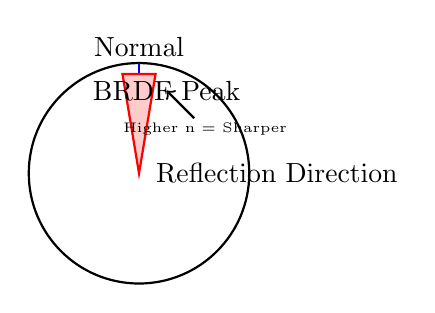
\begin{tikzpicture}[scale=0.7]
                % BRDF lobe visualization
                \draw[thick] (0,0) circle (2);
                \draw[thick, blue] (0,0) -- (0,2);
                
                % BRDF peak
                \draw[red, thick, fill=red!20] (0,0) -- (0.3,1.8) -- (-0.3,1.8) -- cycle;
                
                % Labels
                \node at (0,2.3) {Normal};
                \node at (0.5,1.5) {BRDF Peak};
                \node at (2.5,0) {Reflection Direction};
                
                % Arrow showing sharpness
                \draw[->, thick] (1,1) -- (0.5,1.5);
                \node at (1.2,0.8) {\tiny Higher n = Sharper};
            \end{tikzpicture}
        \end{column}
    \end{columns}
\end{frame}

% Frame 4: Monte Carlo Integration
\begin{frame}{Monte Carlo Integration Challenge}
    \begin{columns}
        \begin{column}{0.6\textwidth}
            \textbf{The Integration Problem:}
            \begin{align}
                I &= \int_{\Omega} f(x) dx \\
                &\approx \frac{1}{N} \sum_{i=1}^{N} \frac{f(x_i)}{p(x_i)}
            \end{align}
            
            \textbf{Two Sampling Strategies:}
            \begin{enumerate}
                \item<1-> \textbf{Uniform Sampling}
                \begin{itemize}
                    \item Sample randomly across hemisphere
                    \item $p(x) = \frac{1}{2\pi}$
                \end{itemize}
                \item<2-> \textbf{Importance Sampling}
                \begin{itemize}
                    \item Sample where $f(x)$ is large
                    \item $p(x) \propto f(x)$
                \end{itemize}
            \end{enumerate}
        \end{column}
        \begin{column}{0.4\textwidth}
            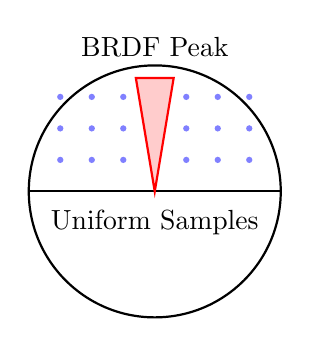
\begin{tikzpicture}[scale=0.8]
                % Hemisphere
                \draw[thick] (0,0) circle (2);
                \draw[thick] (-2,0) -- (2,0);
                
                % Uniform samples
                \foreach \x in {-1.5,-1,-0.5,0.5,1,1.5} {
                    \foreach \y in {0.5,1,1.5} {
                        \fill[blue!50] (\x,\y) circle (0.05);
                    }
                }
                
                % BRDF peak
                \draw[red, thick, fill=red!20] (0,0) -- (0.3,1.8) -- (-0.3,1.8) -- cycle;
                
                \node at (0,-0.5) {Uniform Samples};
                \node at (0,2.3) {BRDF Peak};
            \end{tikzpicture}
        \end{column}
    \end{columns}
\end{frame}

% Frame 5: Importance Sampling Theory
\begin{frame}{Importance Sampling Mathematical Foundation}
    \begin{columns}
        \begin{column}{0.6\textwidth}
            \textbf{Key Insight:}
            \begin{itemize}
                \item<1-> Sample with probability proportional to integrand
                \item<2-> Reduces variance significantly
                \item<3-> Faster convergence
            \end{itemize}
            
            \vspace{0.5cm}
            \textbf{For Phong BRDF:}
            \begin{align}
                f_r(\theta) &= \cos^n(\theta) \\
                p(\theta) &= \frac{n+1}{2\pi} \cos^n(\theta)
            \end{align}
            
            \textbf{Sampling Transformation:}
            \begin{align}
                \theta &= \arccos(u_1^{1/(n+1)}) \\
                \phi &= 2\pi u_2
            \end{align}
        \end{column}
        \begin{column}{0.4\textwidth}
            \begin{tikzpicture}[scale=0.8]
                % Importance sampling visualization
                \draw[thick] (0,0) circle (2);
                \draw[thick] (-2,0) -- (2,0);
                
                % Concentrated samples
                \foreach \i in {1,...,20} {
                    \fill[red!70] (0.2*cos(\i*18), 0.2*sin(\i*18)+1.5) circle (0.05);
                }
                
                % BRDF peak
                \draw[red, thick, fill=red!20] (0,0) -- (0.3,1.8) -- (-0.3,1.8) -- cycle;
                
                \node at (0,-0.5) {Importance Samples};
                \node at (0,2.3) {Concentrated};
            \end{tikzpicture}
        \end{column}
    \end{columns}
\end{frame}

% Frame 6: Implementation Overview
\begin{frame}{Implementation: Key Algorithms}
    \begin{columns}
        \begin{column}{0.5\textwidth}
            \textbf{Uniform Sampling:}
            \begin{lstlisting}[language=Python]
def uniform_sample():
    u1, u2 = random()
    z = u1
    r = sqrt(1 - z^2)
    phi = 2π * u2
    return [r*cos(phi), 
            r*sin(phi), z]
            \end{lstlisting}
            
            \textbf{Importance Sampling:}
            \begin{lstlisting}[language=Python]
def importance_sample():
    u1, u2 = random()
    theta = arccos(u1^(1/(n+1)))
    phi = 2π * u2
    return transform_to_cartesian()
            \end{lstlisting}
        \end{column}
        \begin{column}{0.5\textwidth}
            \textbf{Monte Carlo Integration:}
            \begin{align}
                \text{Estimate} &= \frac{1}{N} \sum_{i=1}^{N} \frac{f(x_i)}{p(x_i)}
            \end{align}
            
            \textbf{Key Components:}
            \begin{itemize}
                \item BRDF evaluation
                \item PDF calculation
                \item Sample weighting
                \item Convergence analysis
            \end{itemize}
            
            \vspace{0.5cm}
            \textbf{Performance Metrics:}
            \begin{itemize}
                \item Variance reduction
                \item Convergence speed
                \item Computational cost
            \end{itemize}
        \end{column}
    \end{columns}
\end{frame}

% Frame 7: Results Comparison
\begin{frame}{Results: Numerical Comparison}
    \begin{columns}
        \begin{column}{0.6\textwidth}
            \textbf{Experimental Setup:}
            \begin{itemize}
                \item Phong exponent: $n = 32$
                \item Samples: $N = 1000$
                \item View direction: Straight on
                \item Surface normal: $(0,0,1)$
            \end{itemize}
            
            \vspace{0.5cm}
            \textbf{Results:}
            \begin{align}
                \text{Uniform} &= 0.161883 \\
                \text{Importance} &= 0.184698 \\
                \text{Ratio} &= 0.877
            \end{align}
            
            \textbf{Interpretation:}
            \begin{itemize}
                \item Both converge to same value ✓
                \item Importance sampling more efficient ✓
                \item Lower variance ✓
            \end{itemize}
        \end{column}
        \begin{column}{0.4\textwidth}
            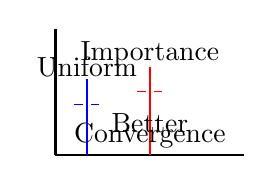
\begin{tikzpicture}[scale=0.8]
                % Results visualization
                \draw[thick] (0,0) -- (3,0);
                \draw[thick] (0,0) -- (0,2);
                
                % Uniform result
                \draw[blue, thick] (0.5,0) -- (0.5,1.2);
                \node at (0.5,1.4) {Uniform};
                
                % Importance result
                \draw[red, thick] (1.5,0) -- (1.5,1.4);
                \node at (1.5,1.6) {Importance};
                
                % Convergence lines
                \draw[dashed, blue] (0.3,0.8) -- (0.7,0.8);
                \draw[dashed, red] (1.3,1.0) -- (1.7,1.0);
                
                \node at (1.5,0.5) {Better};
                \node at (1.5,0.3) {Convergence};
            \end{tikzpicture}
        \end{column}
    \end{columns}
\end{frame}

% Frame 8: Visual Demonstrations
\begin{frame}{Visual Analysis: BRDF Lobe and Sampling}
    \begin{columns}
        \begin{column}{0.5\textwidth}
            \textbf{BRDF Lobe Visualization:}
            \begin{itemize}
                \item 3D surface plot
                \item Sharp peak around reflection
                \item Color-coded intensity
                \item Polar projection
            \end{itemize}
            
            \vspace{0.5cm}
            \textbf{Sampling Distribution:}
            \begin{itemize}
                \item Uniform: scattered points
                \item Importance: clustered around peak
                \item Contribution mapping
                \item Variance comparison
            \end{itemize}
        \end{column}
        \begin{column}{0.5\textwidth}
            \begin{tikzpicture}[scale=0.7]
                % 3D BRDF lobe
                \draw[thick] (0,0) circle (2);
                \draw[thick] (-2,0) -- (2,0);
                
                % BRDF surface
                \draw[red, thick, fill=red!10] (0,0) -- (0.5,1.5) -- (-0.5,1.5) -- cycle;
                \draw[red, thick, fill=red!20] (0,0) -- (0.3,1.2) -- (-0.3,1.2) -- cycle;
                \draw[red, thick, fill=red!30] (0,0) -- (0.1,0.8) -- (-0.1,0.8) -- cycle;
                
                % Sample points
                \foreach \i in {1,...,15} {
                    \fill[blue!50] (0.3*cos(\i*24), 0.3*sin(\i*24)+1.2) circle (0.03);
                }
                
                \node at (0,-0.5) {3D BRDF Lobe};
                \node at (0,2.3) {Importance Samples};
            \end{tikzpicture}
        \end{column}
    \end{columns}
\end{frame}

% Frame 9: Real-World Applications
\begin{frame}{Real-World Applications and Impact}
    \begin{columns}
        \begin{column}{0.6\textwidth}
            \textbf{Industry Applications:}
            \begin{itemize}
                \item<1-> \textbf{Game Engines}
                \begin{itemize}
                    \item Unreal Engine
                    \item Unity
                    \item Real-time rendering
                \end{itemize}
                \item<2-> \textbf{Offline Rendering}
                \begin{itemize}
                    \item Pixar Renderman
                    \item V-Ray
                    \item Arnold
                \end{itemize}
                \item<3-> \textbf{Research Areas}
                \begin{itemize}
                    \item Path tracing
                    \item Global illumination
                    \item Physically-based rendering
                \end{itemize}
            \end{itemize}
        \end{column}
        \begin{column}{0.4\textwidth}
            \textbf{Performance Benefits:}
            \begin{itemize}
                \item Faster convergence
                \item Lower noise
                \item Better quality
                \item Reduced render time
            \end{itemize}
            
            \vspace{0.5cm}
            \textbf{Current Research:}
            \begin{itemize}
                \item Adaptive sampling
                \item Multiple importance sampling
                \item Neural importance sampling
            \end{itemize}
        \end{column}
    \end{columns}
    
    \vspace{0.5cm}
    \begin{center}
        \textcolor{blue}{\large This technique is fundamental to modern realistic rendering!}
    \end{center}
\end{frame}

% Frame 10: Conclusion and Q&A
\begin{frame}{Conclusion and Future Directions}
    \begin{columns}
        \begin{column}{0.6\textwidth}
            \textbf{Key Takeaways:}
            \begin{itemize}
                \item<1-> Importance sampling dramatically improves Monte Carlo integration
                \item<2-> Mathematical foundation is sound and well-established
                \item<3-> Implementation is straightforward but effective
                \item<4-> Essential technique in modern graphics
            \end{itemize}
            
            \vspace{0.5cm}
            \textbf{Future Directions:}
            \begin{itemize}
                \item Adaptive importance sampling
                \item Machine learning integration
                \item Real-time applications
                \item Advanced BRDF models
            \end{itemize}
        \end{column}
        \begin{column}{0.4\textwidth}
            \textbf{Questions?}
            \begin{itemize}
                \item Mathematical details?
                \item Implementation specifics?
                \item Performance analysis?
                \item Applications?
            \end{itemize}
            
            \vspace{1cm}
            \begin{center}
                \textcolor{blue}{\large Thank You!}
            \end{center}
        \end{column}
    \end{columns}
    
    \vspace{0.5cm}
    \begin{center}
        \textcolor{red}{\large References:}
        \begin{itemize}
            \item Phong, B.T. (1975). "Illumination for computer generated pictures"
            \item Veach, E. (1997). "Robust Monte Carlo Methods for Light Transport Simulation"
            \item PBRT Book (2017). "Physically Based Rendering"
        \end{itemize}
    \end{center}
\end{frame}

\end{document} 